% This is auto-generated file: do not edit!
% Exported from microMathematics Plus, version 2.17.0


Dieses Beispiel demonstriert 3D Plots
zu drei verschiedenen Funktionen
zweier Variablen.

Zuerst definieren wir Intervalle für
x- und y-Argumente. Das Intervall der
x-Achse hängt von der Anzahl der
Punkte entlang der x-Achse sowie den
Minimal- und Maximalwerten x1 und x2
ab:
\begin{center}\begin{tabular}{ccc}
  $N := 300$ &
  $x1 := -2$ &
  $x2 := 2$ \cr
\end{tabular}\end{center}
\begin{center}\begin{tabular}{c}
  $x := \left[ x1,\, x1 +  \left| x2 - x1 \right|  / N \,..\, x2 \right]$
\end{tabular}\end{center}

Das Intervall für die y-Achse wird dem
entsprechend definiert:
\begin{center}\begin{tabular}{ccc}
  $M := 300$ &
  $y1 := -3$ &
  $y2 := 3$ \cr
\end{tabular}\end{center}
\begin{center}\begin{tabular}{c}
  $y := \left[ y1,\, y1 +  \left| y2 - y1 \right|  / M \,..\, y2 \right]$
\end{tabular}\end{center}

Wir zeichnen nun als Beispiel eine
trigonometrische Funktion, die ein
Produkt von Sinus und Kosinus ist:
\begin{center}\begin{tabular}{c}
  $F(x,y) := sin \left( 3 \cdot {x}^{2}\right)  \cdot cos \left( {y}^{2}\right) $
\end{tabular}\end{center}

Für die 3D Ansicht klicken Sie auf ''3D
Plot hinzufügen'' in der Werkzeugleiste
oder ''Neu'' in der Menüleiste:
\begin{center}\begin{tabular}{c} 
\includegraphics[resolution=320]{graphics/three_d_plot_fig1.png} \end{tabular}\end{center}

Setzen Sie den Funktionsnamen F(x,y) in
das untere Mittelfeld:
\begin{center}\begin{tabular}{c} 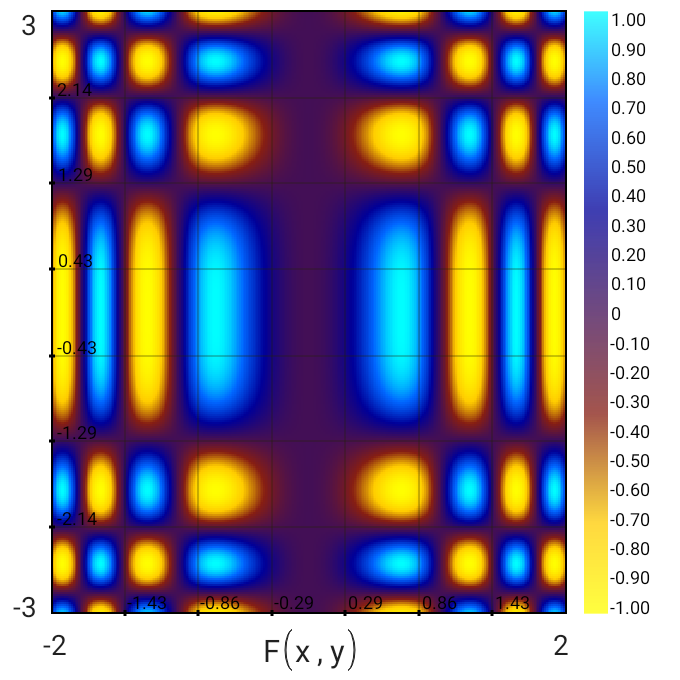
\includegraphics[resolution=320]{graphics/three_d_plot_fig2.png} \end{tabular}\end{center}

Plot Grenzen, Größe, Stil, Bezeichnung
und Raster können mittels des
Dialogfensters ''Plot Einstellungen''
angepasst werden (siehe das Beispiel
zu ''Plot einer Funktion'' im Hauptmenü
für mehr Informationen). Wenn Sie auf
die Mitte des Plot Bereichs lange
gedrückt halten, erscheint ein Action
Button ''Objekteinstellungen''. Ein Tap
auf diesen Button öffnet dieses
Dialogfenster.

Zudem können Sie die Anzahl der
Bezeichnungen entlang der z-Achse
ändern und die Farbenpalette im Dialog
''Farbtabellen Einstellungen'' wählen.
Dieser Dialog erscheint ebenfalls
durch langes Drücken der z-Achse im
rechten Bereich des Hauptgraphen.
\begin{center}\begin{tabular}{c}
  $R(x,y) := sin \left( 5 \cdot {x}^{2} \cdot \left( y - x \right)\right) $
\end{tabular}\end{center}
\begin{center}\begin{tabular}{c} 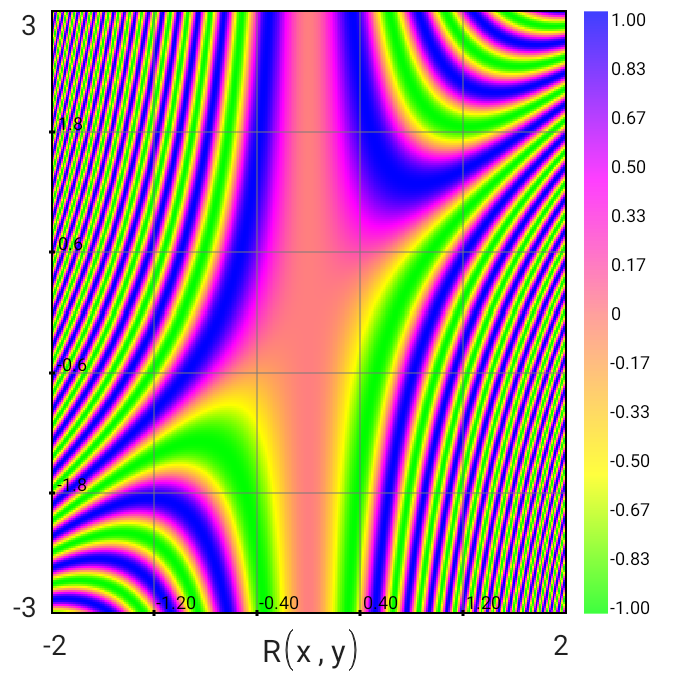
\includegraphics[resolution=320]{graphics/three_d_plot_fig3.png} \end{tabular}\end{center}

Eine Funktion zweier Argumente kann
ebenso als Oberfläche im
dreidimensionalen Raum aufgetragen
werden. Dieser Modus kann in den ''Plot
Einstellungen'' Dialog aktiviert
werden, indem man den Button
''Objekteinstellungen'' clickt, der
durch langes Gedrückthalten auf die
Mitte des Plot Bereichs erscheint. Um
die Berechnungszeit zu verbessern,
verwenden wir Arrays und zeichnen nun
die folgende Funktion F(n,m):
\begin{center}\begin{tabular}{cccc}
  $N := 100$ &
  $n := \left[ 0,\, 1 \,..\, N \right]$ &
  $x1 := -15$ &
  $x2 := 15$ \cr
\end{tabular}\end{center}
\begin{center}\begin{tabular}{cccc}
  $M := 100$ &
  $m := \left[ 0,\, 1 \,..\, M \right]$ &
  $y1 := -15$ &
  $y2 := 15$ \cr
\end{tabular}\end{center}
\begin{center}\begin{tabular}{c}
  $x[n] := {\left( x1 +  \left( x2 - x1\right)  \cdot n / N \right)}^{2}$
\end{tabular}\end{center}
\begin{center}\begin{tabular}{c}
  $y[m] := {\left( y1 +  \left( y2 - y1\right)  \cdot m / M \right)}^{2}$
\end{tabular}\end{center}
\begin{center}\begin{tabular}{c}
  $r[n,m] := 0.04 \cdot x_{n}  + 0.02 \cdot y_{m} $
\end{tabular}\end{center}
\begin{center}\begin{tabular}{c}
  $t[n,m] := \left( x_{n}  + 0.05 \cdot y_{m}  \right) \cdot exp \left( 1 - r_{n,\, m} \right) $
\end{tabular}\end{center}
\begin{center}\begin{tabular}{c}
  $F[n,m] := \frac{sin \left( x_{n}  + 0.1 \cdot y_{m} \right) }{0.15 + r_{n,\, m} } + \frac{t_{n,\, m} }{10}$
\end{tabular}\end{center}
\begin{center}\begin{tabular}{c} 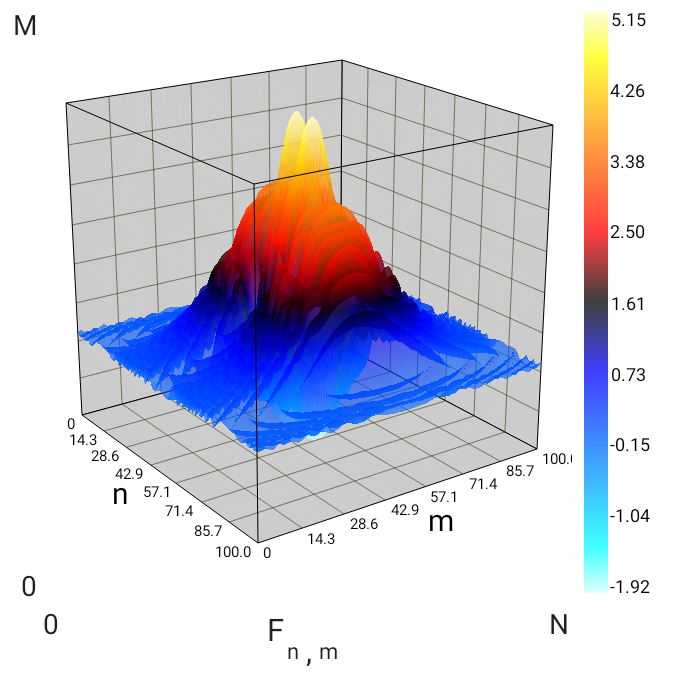
\includegraphics[resolution=320]{graphics/three_d_plot_fig4.png} \end{tabular}\end{center}

Um die Plot Oberfläche zu gestalten
gibt es zusätzliche Einstellungen, die
im Dialog ''Plot Einstellungen'' zu
finden sind. Sie können wählen, ob die
Netzlinien sichtbar sein sollen,
welche Deckkraft deren Farbe haben
soll, oder die Rotations- und
Elevationswinkel der Plot Box
definieren. Zum Beispiel, die oben
gezeigte Oberfläche sieht aus der
anderen Perspektive so aus: 
\begin{center}\begin{tabular}{c} 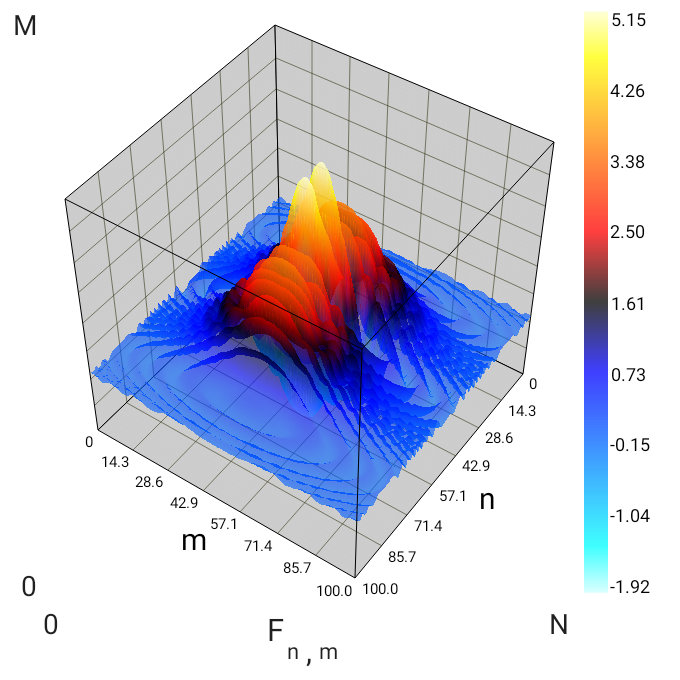
\includegraphics[resolution=320]{graphics/three_d_plot_fig5.png} \end{tabular}\end{center}